%%%%%%%%%%%%%%%%%%%%%%%%%%%%%%%%%%%%%%%%%%%%%%%%%%%%%%%%%%%%%%%%%%%%%%%%%%%%%%%%
% PREAMBLE
%%%%%%%%%%%%%%%%%%%%%%%%%%%%%%%%%%%%%%%%%%%%%%%%%%%%%%%%%%%%%%%%%%%%%%%%%%%%%%%%
\documentclass[12pt, a4paper, ukenglish]{article}

% -------------------------- Font and Encoding ---------------------------------
\usepackage[T1]{fontenc}
\usepackage{times} % Use Times font
\usepackage[utf8]{inputenc}

% -------------------------- Page Layout ---------------------------------------
\usepackage[left=2.5cm, top=2cm, right=2.5cm, bottom=2cm]{geometry}
\setlength{\parskip}{\medskipamount}

% -------------------------- Required Packages ---------------------------------
\usepackage{amsmath}
\usepackage{amssymb}
\usepackage{graphicx}
\usepackage{cancel}
\usepackage{esint}
\usepackage{mathdots}
\usepackage{mathtools}
\usepackage[version=4]{mhchem}
\usepackage{stackrel}
\usepackage{stmaryrd}
% \usepackage{undertilde}
\usepackage{longtable}
\usepackage{booktabs}
\usepackage{pdfpages}
% \usepackage[ukenglish]{babel}

% -------------------------- Bibliography Settings -----------------------------
% NOTE: The 'cite' package conflicts with biblatex. It has been removed.
\usepackage[style=ieee, backend=biber]{biblatex}
\addbibresource{final_report.bib} % Make sure this filename matches your .bib file

% -------------------------- Hyperlinks Settings -------------------------------
\usepackage{xcolor} % Colours for hyperref package
% Define links colour
\newcommand{\linksColour}{black}
% hyperref package
\usepackage[colorlinks=true, linkcolor=\linksColour, citecolor=\linksColour, urlcolor=blue, bookmarksnumbered=true, bookmarksopen=true, bookmarksopenlevel=1]{hyperref}
% \usepackage{breakurl}      % break long urls
\urlstyle{rm}               % Change url fonts to match report font

% -------------------- Header and Footer Settings ------------------------------
\usepackage{fancyhdr}
\pagestyle{fancy}
\fancyhead{}                   % clear the default header
\fancyfoot{}                   % clear the default footer
% \fancyfoot[CO,CE]{\footnotesize\thepage}   % page number in the middle
\renewcommand{\headrulewidth}{0.0pt}       % remove the default header line
% Header and footer of automatically generated pages (e.g. TOC)
\fancypagestyle{plain}{
    \fancyhead{}
    \fancyfoot{}
    % \fancyfoot[CO,CE]{\footnotesize\thepage}
    \renewcommand{\headrulewidth}{0pt}
}

% ------------------------ Title Page Box Settings -----------------------------
% settings for the text box on the front page
\newcommand\HRule{\noindent\rule{\linewidth}{2pt}}

% -------------------------- Figures Settings ----------------------------------
% Redefine how latex deals with figure placement
\renewcommand{\topfraction}{.85}
\renewcommand{\bottomfraction}{.7}
\renewcommand{\textfraction}{.15}
\renewcommand{\floatpagefraction}{.66}
\renewcommand{\dbltopfraction}{.66}
\renewcommand{\dblfloatpagefraction}{.66}
\usepackage[labelfont={bf,footnotesize},textfont={footnotesize}, labelsep=quad]{caption}

% ------------------------------ TOC Settings ----------------------------------
% Adding dots to sections in table of contents
\usepackage{tocloft}
\renewcommand{\cftloftitlefont}{\large\bfseries}
\renewcommand{\cftlottitlefont}{\large\bfseries}
\renewcommand{\cftsecleader}{\cftdotfill{\cftdotsep}}
% Adding the word Figure in list of figures
\renewcommand*\cftfigpresnum{Figure~}
\settowidth{\cftfignumwidth}{\cftfigpresnum}
\renewcommand{\cftfigaftersnumb}{\qquad}
% Adding the word Table in list of figures
\renewcommand*\cfttabpresnum{Table~}
\settowidth{\cfttabnumwidth}{\cfttabpresnum}
\renewcommand{\cfttabaftersnumb}{\qquad}
\setcounter{secnumdepth}{3}
\setcounter{tocdepth}{3}

% -------------------- Formatting Section Titles -------------------------------
% Shrinking the space after headers
\usepackage[clearempty]{titlesec} % loaded with a setting for automatically generated empty pages to be completely blank
\beforetitleunit = 1pt
\aftertitleunit = 1pt
% specifying the spacing before and after the titles (note \parskip = 9pts)
\titlespacing{\section}{0pt}{*9}{*9}    % for 18 pt space
\titlespacing{\subsection}{0pt}{*3}{*3}  % for 12 pt space
\titlespacing{\subsubsection}{0pt}{*3}{*3} % for 12 pt space
% specifying the title formatting
\titleformat{\section} {\normalfont\fontsize{14}{14}\bfseries}{\thesection.}{1em}{}
\titleformat{\subsection} {\normalfont\fontsize{12}{12}\bfseries}{\thesubsection}{1em}{}
\titleformat{\subsubsection} {\normalfont\fontsize{12}{12}\it}{\thesubsubsection}{1em}{}

% Modifying how appendices look (title and toc)
\usepackage[titletoc,title]{appendix}

% ------------------------- Nomenclature Settings ------------------------------
\usepackage{nomencl}
\makenomenclature
\def\nompreamble{\addcontentsline{toc}{section}{\nomname}\markboth{\nomname}{\nomname}}
% customising nomenclature groups
\usepackage{ifthen}
\renewcommand{\nomgroup}[1]{
    \ifthenelse{\equal{#1}{A}}{\item[\textbf{Symbols}]}{%
    \ifthenelse{\equal{#1}{G}}{\item[\textbf{Greek Symbols}]}{}
    }% matches Greek Symbols
}% matches Roman Symbols
% unit column in nomenclature
\newcommand{\nomunit}[1]{\renewcommand{\nomentryend}{\hspace*{\fill}#1}}

% -------------------------- Code Listings Settings ----------------------------
\usepackage{listings}
\lstset{
    basicstyle={\ttfamily\footnotesize},
    belowcaptionskip=3mm,
    breaklines=true,
    commentstyle={\color[rgb]{0,0.5,0}},
    frame=tb, % Top and bottom frame lines
    keywordstyle={\color{blue}},
    language=Matlab,
    numbers=left,
    numberstyle={\scriptsize},
    showstringspaces=false,
    stringstyle={\color{purple}}
}
% Change default name for code environments
\renewcommand{\lstlistingname}{Program}

% -------------------------- Miscellaneous Settings ----------------------------
\usepackage[british]{isodate}
\usepackage{menukeys}       % for menu instructions
\usepackage[bottom]{footmisc} % force footnotes to be always at the bottom of the page
\usepackage{multirow}
\usepackage{units}
\allowdisplaybreaks     % to allow page breaks within equations

% Disable automatic date printing
% \date{}


%%%%%%%%%%%%%%%%%%%%%
% REFERENCING OF IMAGES AND FIGURE
%%%%%%%%%%%%%%%%%%%%%%%%

%%%%%%%%%%%%%%%%%%%%%%%%
% IMAGES
%%%%%%%%%%%%%%%%%%%%%%%%
\newcommand{\catImage}{
    \begin{figure}[h!]
        \centering
        
\includegraphics[width=0.3\linewidth]{figures/cat.jpg}
        \caption{Image of a cat used for testing the AlexNet model}
        \label{fig:cat}
    \end{figure}
}
%%%%%%%%%%%%%%%%%%%%%%%%
% FIGURES
%%%%%%%%%%%%%%%%%%%%%%%%
\newcommand{\MACRegImage}{
    \begin{figure}[h!]
        \centering
        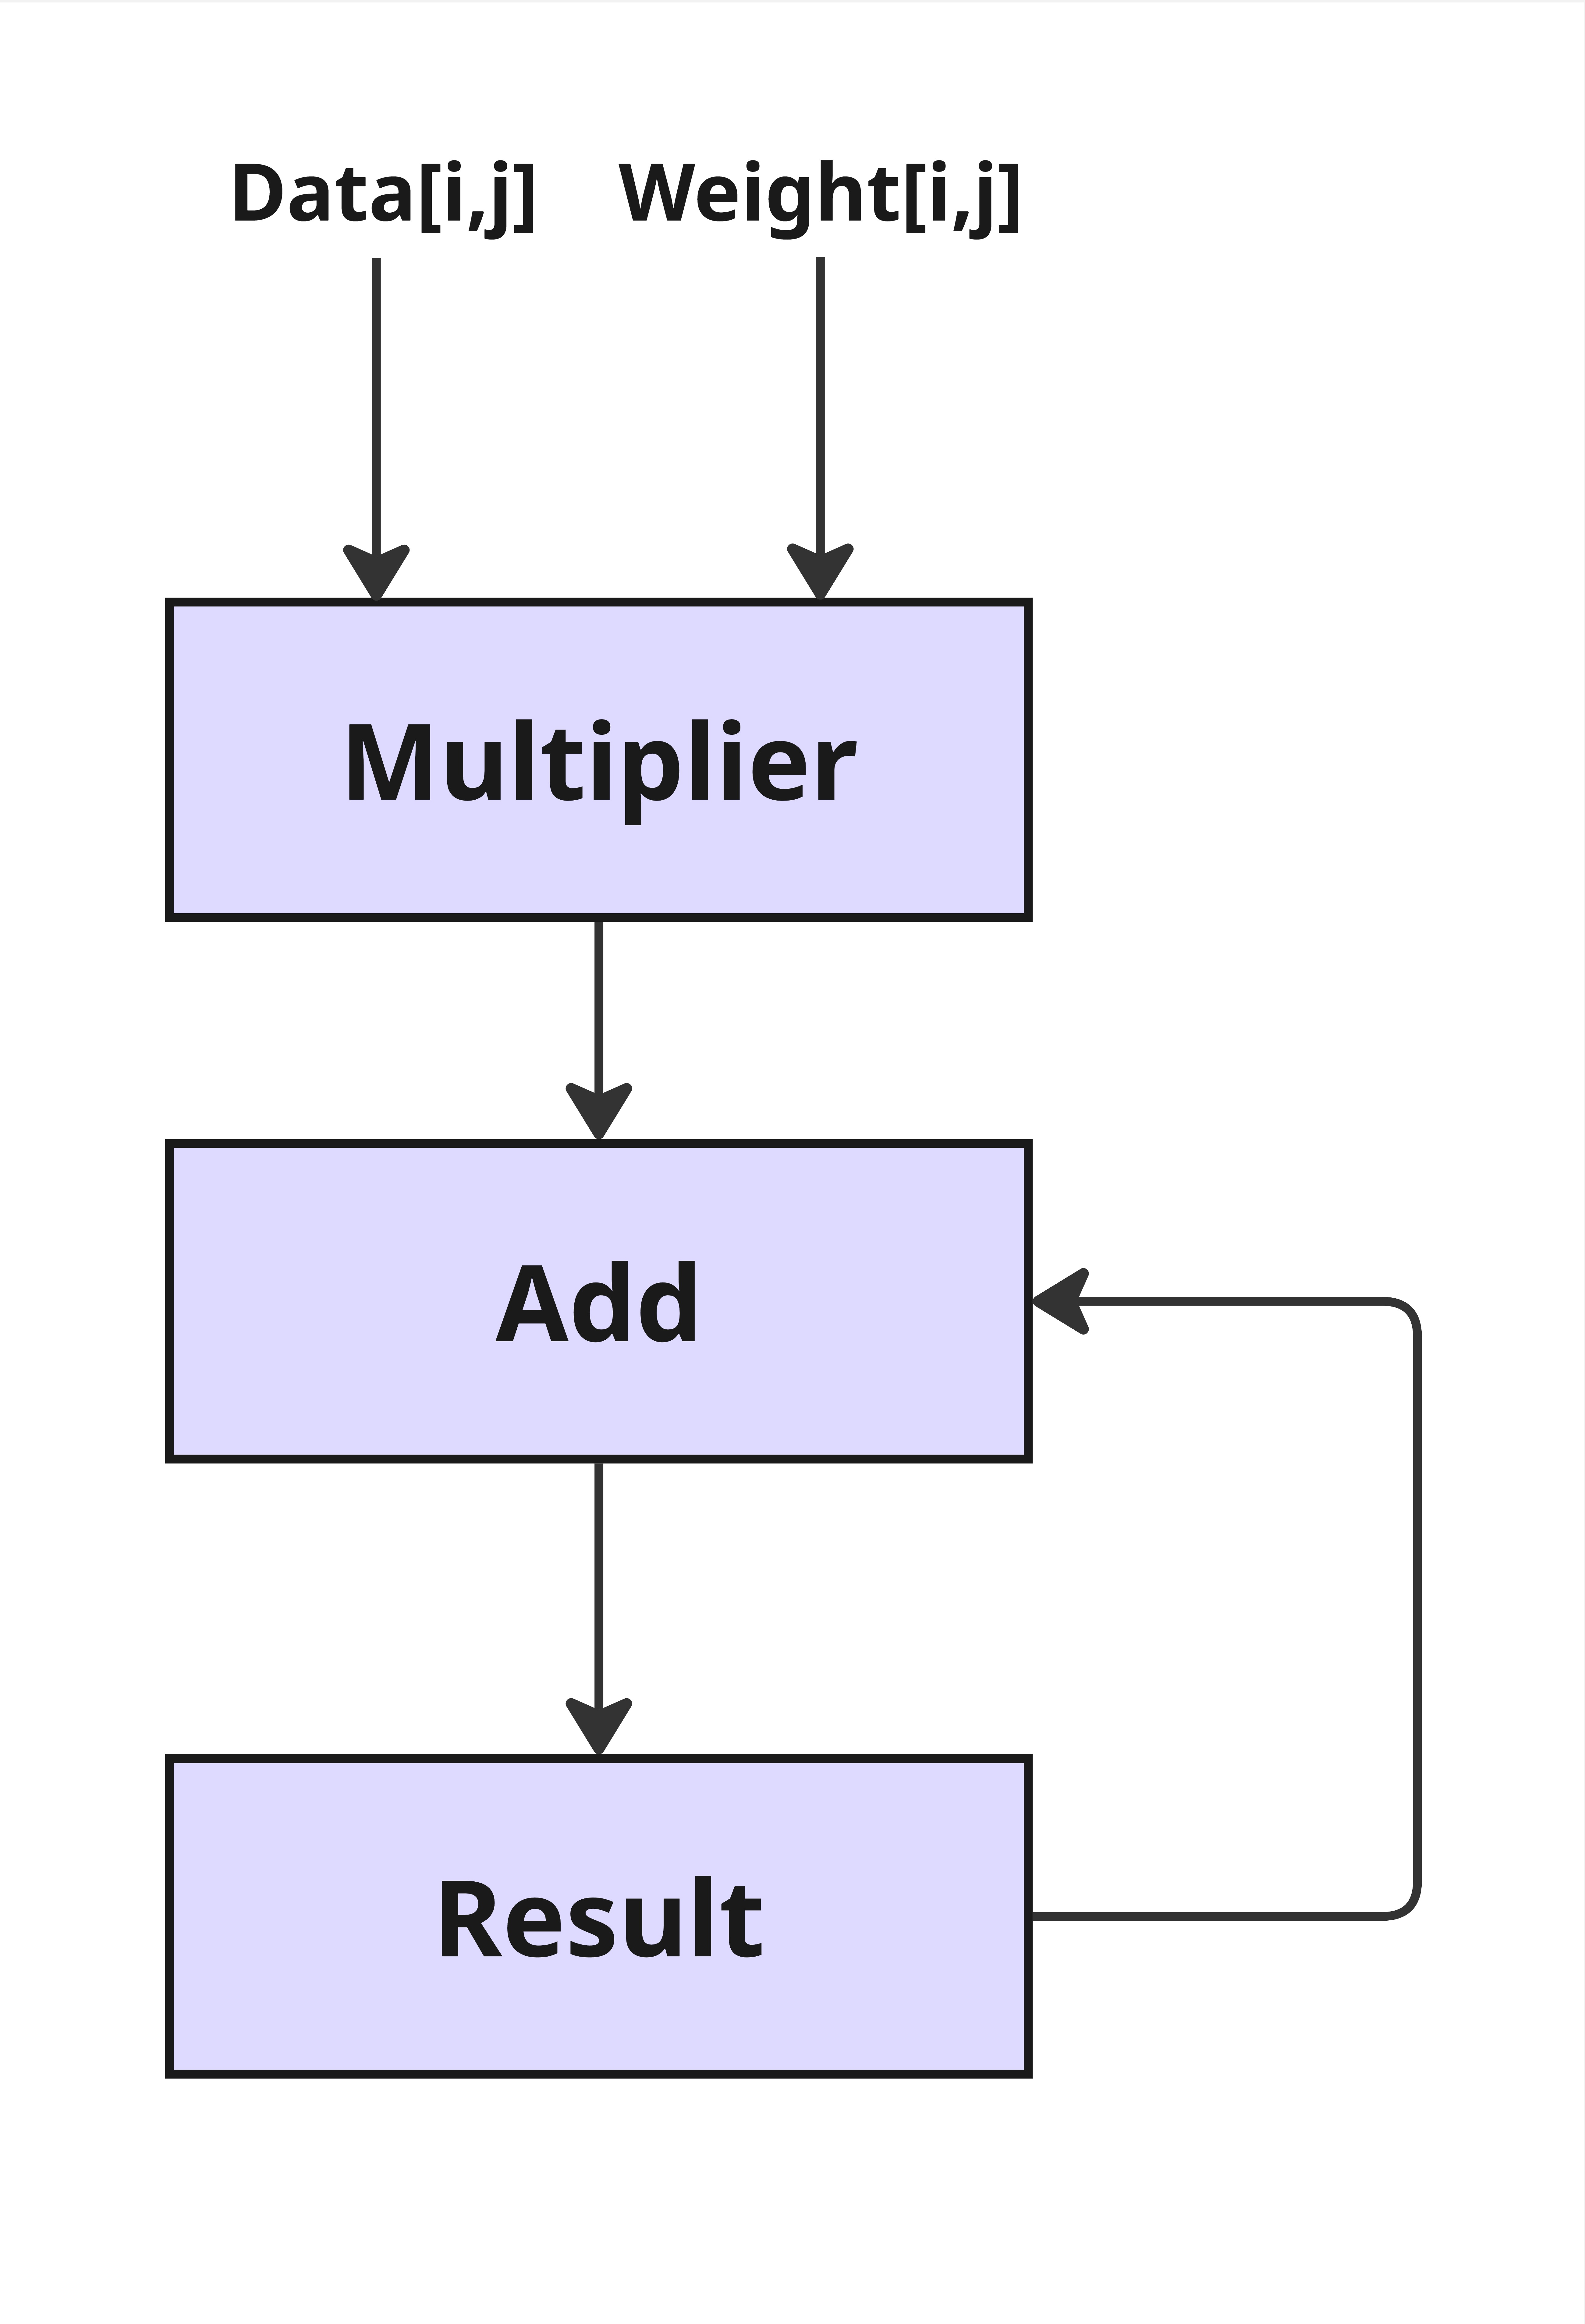
\includegraphics[width=0.2\linewidth]{figures/MAC.jpg}
        \caption{Image of the MAC unit in the Processing Element (PE)}
        \label{fig:MAC}
    \end{figure}
}
\newcommand{\baselineSystolicArrayImage}{
    \begin{figure}[h!]
        \centering
        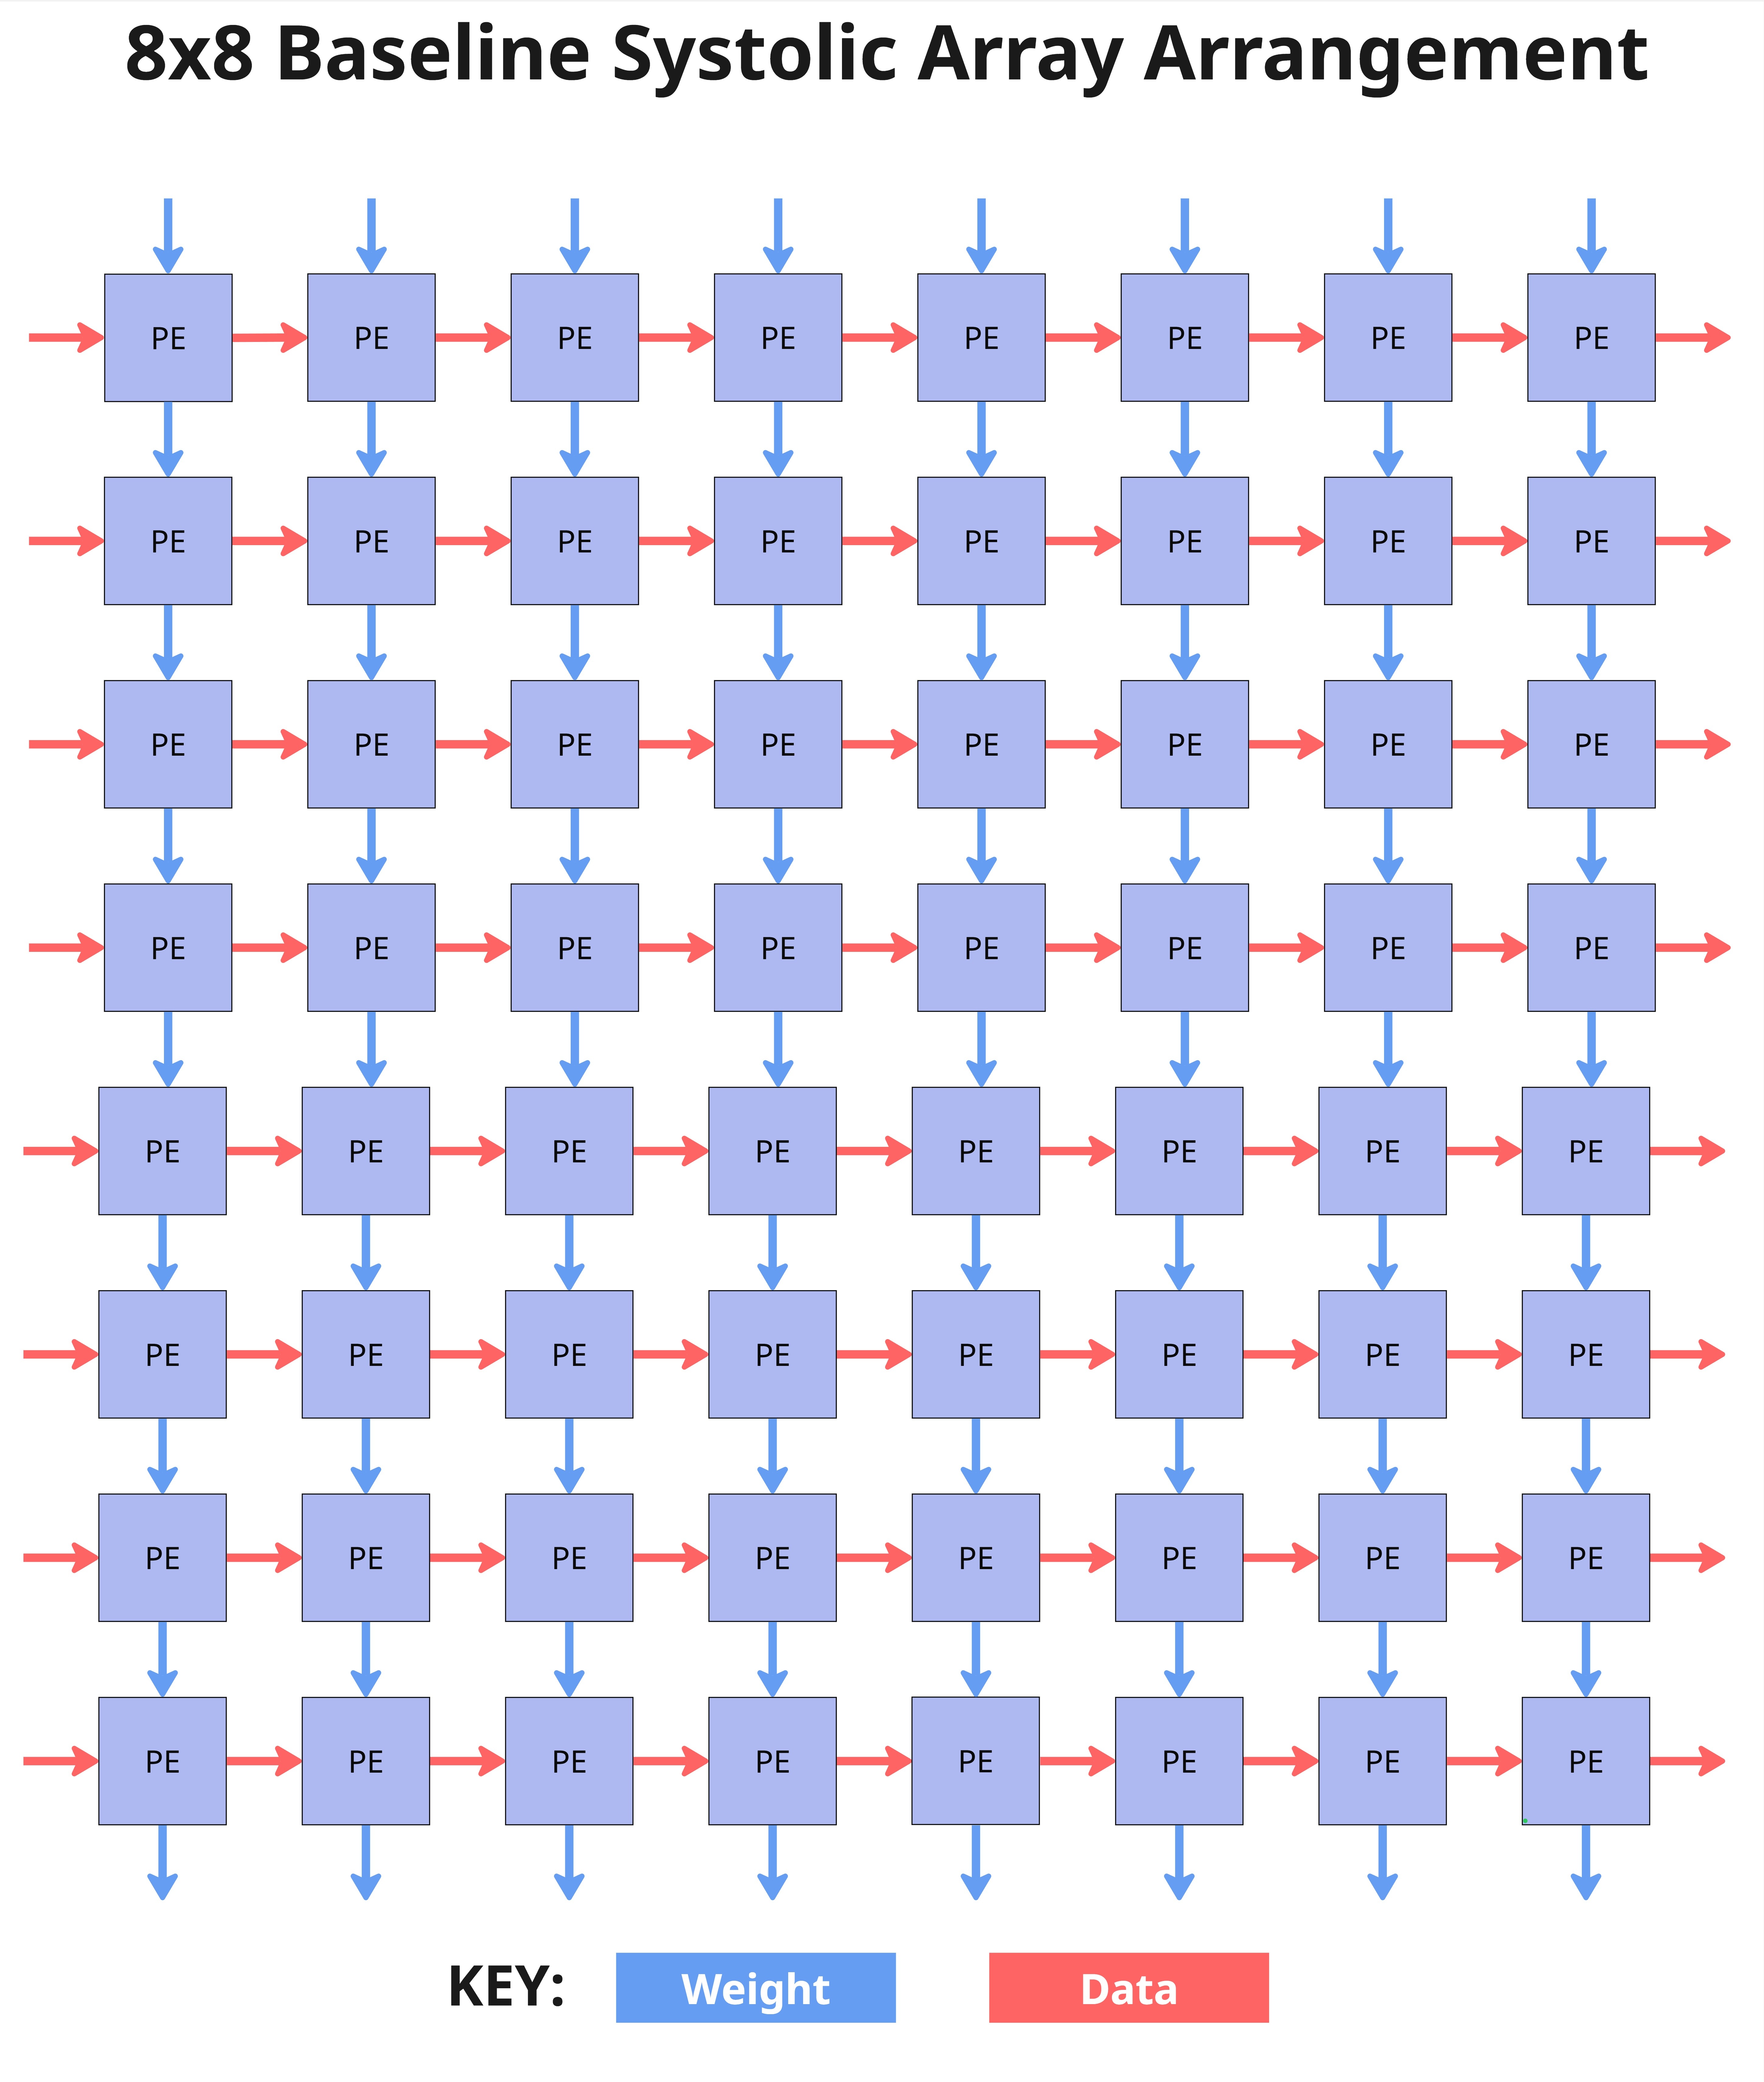
\includegraphics[width=0.5\linewidth]{figures/baseline_systolic_array.jpg}
        \caption{Image of the Baseline Systolic Array Arragement}
        \label{fig:baseline_systolic_array}
    \end{figure}
}

\newcommand{\baselineDataflowImage}{
    \begin{figure}[h!]
        \centering
        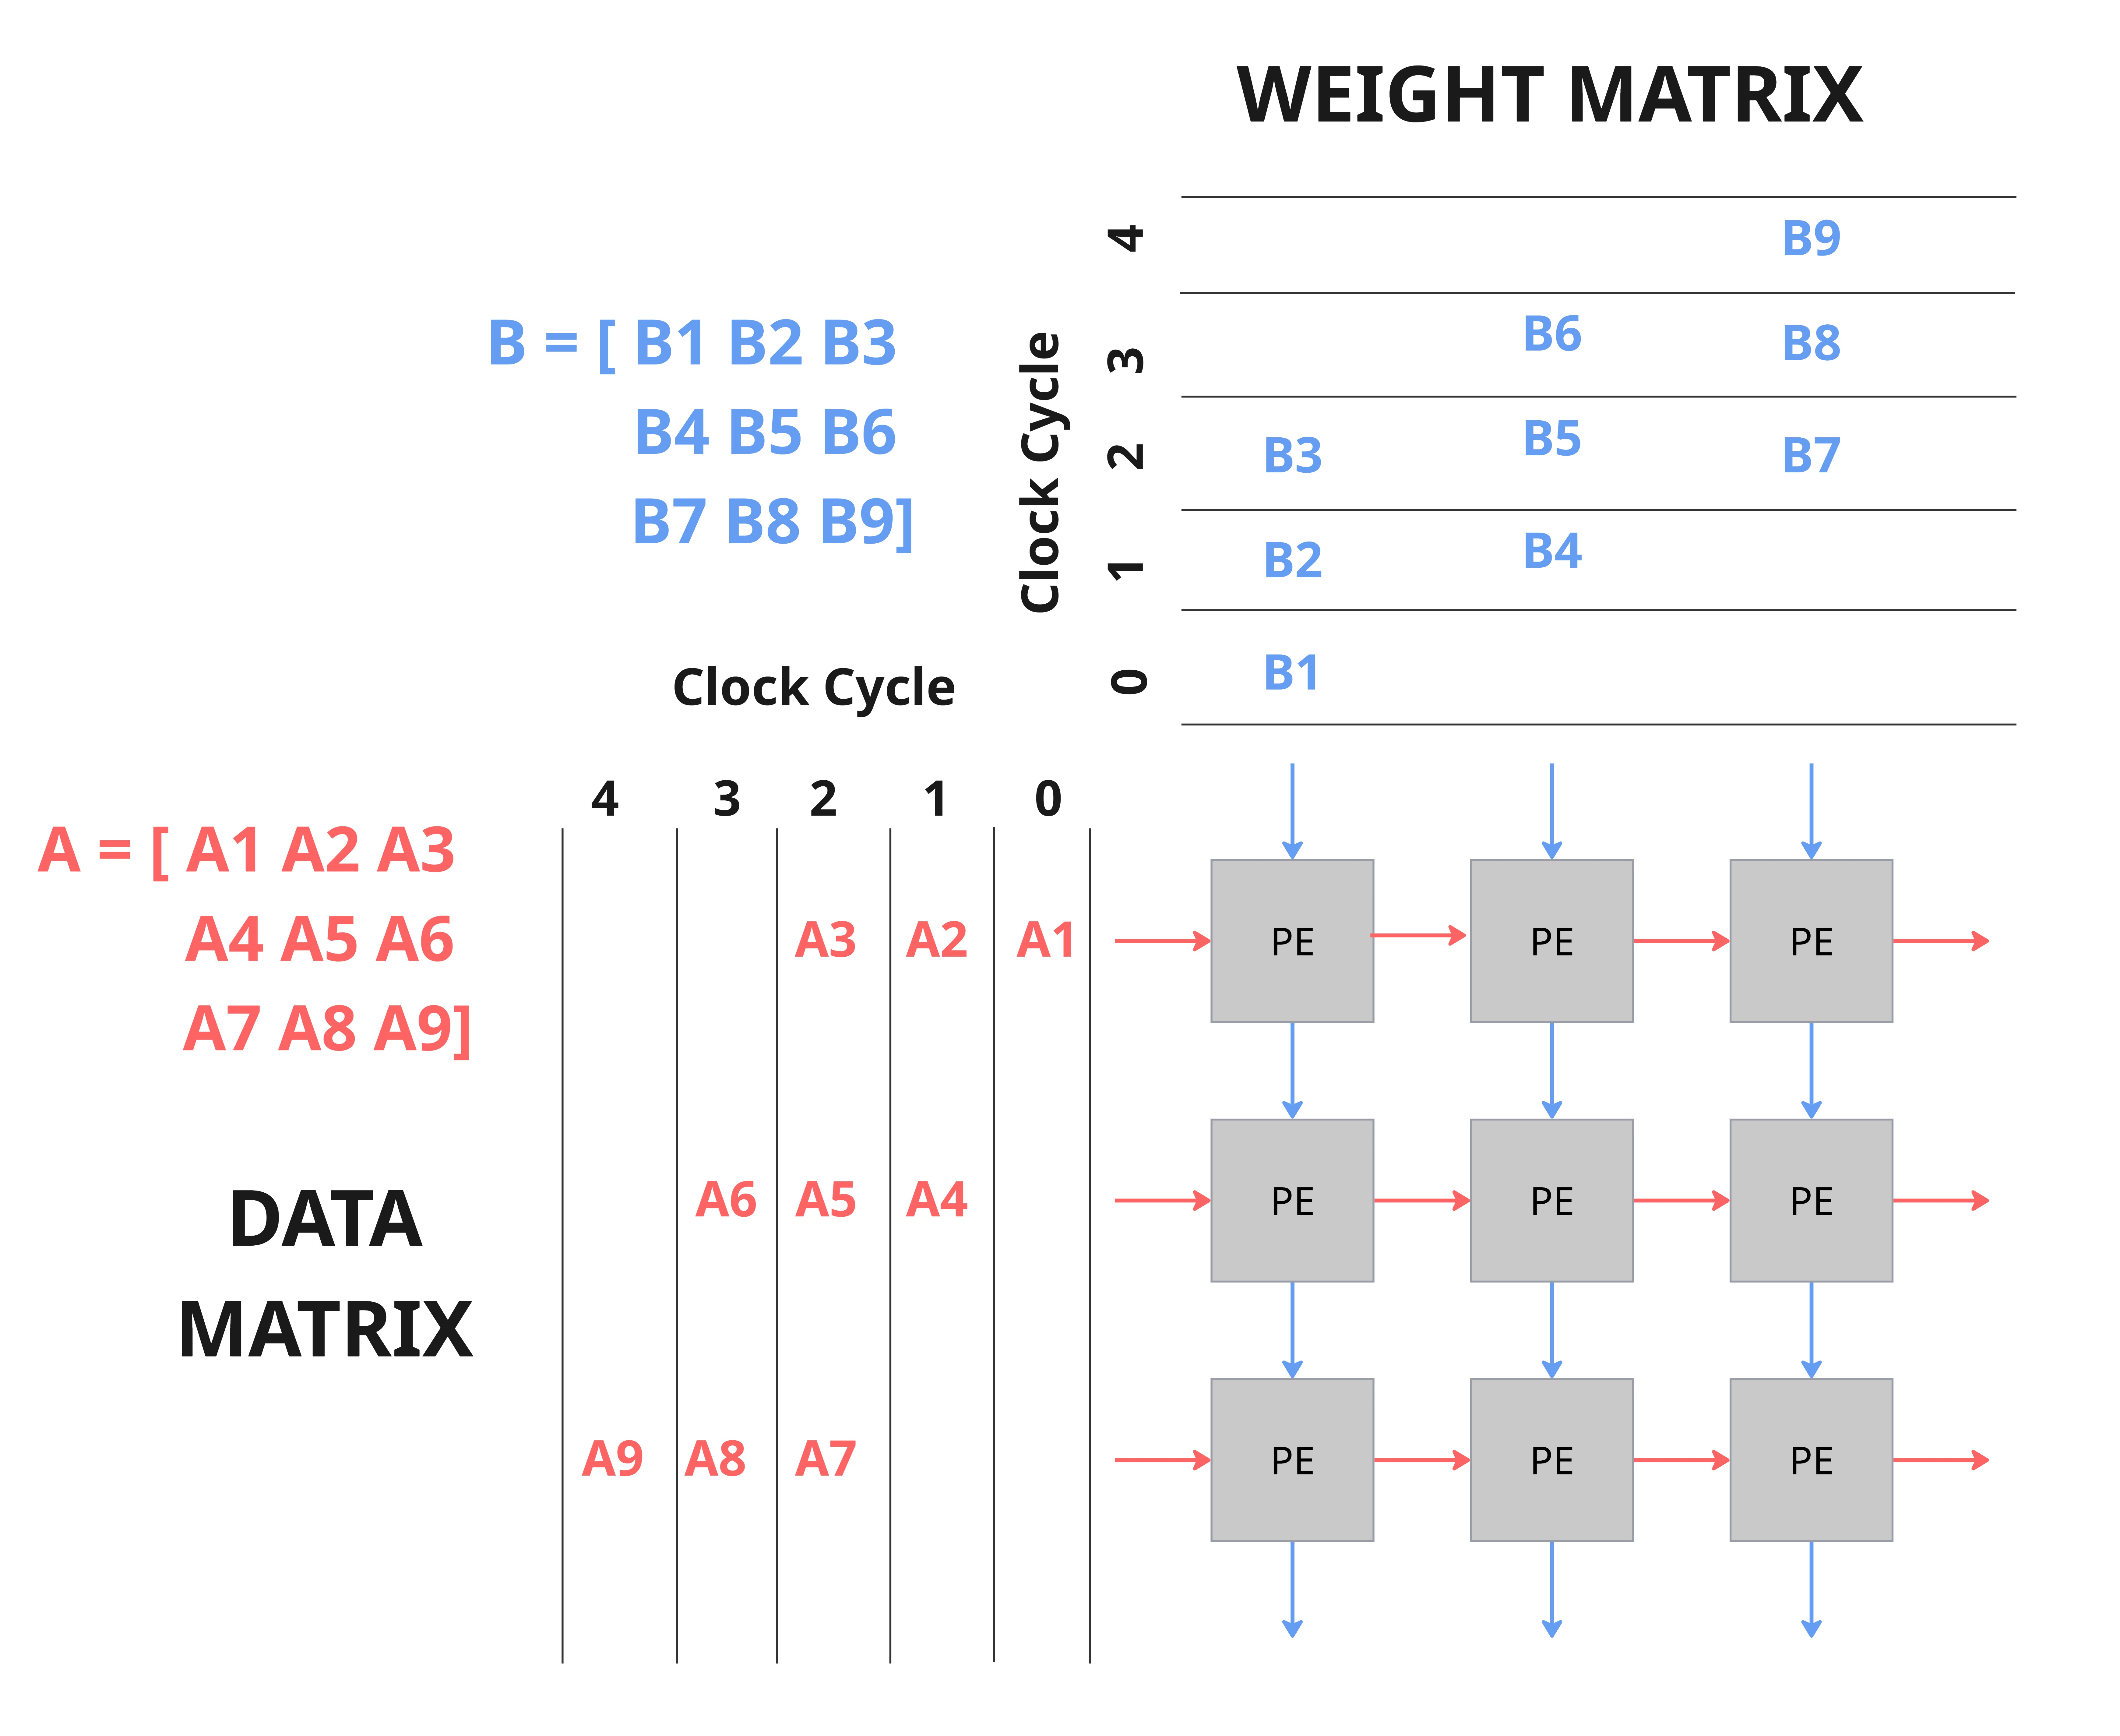
\includegraphics[width=0.5\linewidth]{figures/baseline_systolic_array_dataflow.jpg}
        \caption{Image of the Baseline Systolic Array's Dataflow}
        \label{fig:baseline_dataflow}
    \end{figure}
}




% add page numbers
\fancyfoot[CO,CE]{\footnotesize\thepage}   % page number  
% line spacing 
\usepackage{setspace}
\setstretch{1.15}





%%%%%%%%%%%%%%%%%%%%%%%%%%%%%%%%%%%%%%%%%%%%%%%%%%%%%%%%%%%%%%%%%%%%%%%%%%%%%%%%
% DOCUMENT BODY
%%%%%%%%%%%%%%%%%%%%%%%%%%%%%%%%%%%%%%%%%%%%%%%%%%%%%%%%%%%%%%%%%%%%%%%%%%%%%%%%
\begin{document}

% --- Define name and report number he
\def\name{Kristelle Sampang}
\def\reportNumber{COMPSYS043-\the\year}

% --- Title Page ---
\thispagestyle{empty}
\pagenumbering{roman}

\begin{center}
    \vspace*{10mm}
    % {\large \textbf{Research Project in Computer Systems Engineering}}

    \vspace*{10mm}
    \HRule
    
    \vspace{0.5cm}
    Final Report
    \vspace{0.5cm}
    
    {\Large \textbf{Project \#43: Reconfigurable Neural Processing Unit (NPU) for Energy-Efficient AI at the Edge}}
    
    \vspace{1cm}
    {\large \name}
    
    \vspace{0.5cm}
    Project Report 
    
    \vspace{0.5cm}
    \HRule
\end{center}

\vfill
\begin{center}
    \begin{tabular}{r l}
        \addlinespace[1.5em]
        Project Partner: & Pratham Chhabra \\
        \addlinespace[1.5em]
        Supervisor: & Dr Morteza Biglari-Abhari \\
        \addlinespace[1.5em]
        Co-Supervisor: & Dr Maryam Hemmati
    \end{tabular}
\end{center}

\vfill
\begin{center}
    \today
\end{center}

\vfill
\begin{center}
    % \includegraphics[width=0.7\linewidth]{figures/ecse-horizontal-hc.png}
    
\includegraphics[width=0.4\linewidth]{figures/UoA-Logo-Primary-RGB-Large.png}
\end{center}

\clearpage

% --- Abstract Page ---
\noindent \reportNumber

\vspace{1em}
\begin{center}
    {\large \textbf{\scshape Reconfigurable Neural Processing Unit (NPU) for Energy-Efficient AI at the Edge}}
\end{center}

\vspace{2em}
\begin{center}
    {\large \textbf{\name}}
\end{center}

\vspace{2em}
\begin{center}
    {\large \textbf{\scshape ABSTRACT}}
\end{center}

Abstract goes here.

% --- Declaration Page ---
% \includepdf[pages=-, pagecommand={\thispagestyle{fancy}}]{Declaration.pdf}
\clearpage
\newpage
\vspace{2em}
\begin{center}
\Large\textbf{DECLARATION}
\end{center}
\noindent
\textbf{Student}
\vspace{1em}
I hereby declare that:
\begin{enumerate}
    \item This report is the result of the final year project work carried out by my project partner (see cover page) and I under the guidance of our supervisor (see cover page) in the 2025 academic year at the Department of Electrical, Computer and Software Engineering, Faculty of Engineering, University of Auckland. 
    \item This report is not the outcome of work done previously. 
    \item This report is not the outcome of work done in collaboration, except that with a potential project sponsor (if any) as stated in the text.
    \item This report is not the same as any report, thesis, conference article or journal paper, or any other publication or unpublished work in any format. 
\end{enumerate}
\vspace{1em}
\noindent
In the case of a continuing project, please state clearly what has been developed during the project and what was available from previous year(s): 
\vspace{3cm}
\noindent
\newline
Signature:

\includegraphics[width=0.3\linewidth]{figures/signature.png}

\vspace{1cm}
Date: 
\includegraphics[width=0.2\linewidth]{figures/date.png}
% !! Remember to sign this

\newpage

% --- Table of Contents ---
\setlength{\parskip}{6pt}
\renewcommand{\contentsname}{\large{Table of Contents}}
\tableofcontents
\newpage
\setlength{\parskip}{9pt}

% --- Acknowledgements ---
\section*{Acknowledgements}
\addcontentsline{toc}{section}{Acknowledgements}

\label{sec:Acknowledgements1}

Thank important people here.



\newpage

% --- Glossary of Terms ---
\section*{Glossary of Terms}
\addcontentsline{toc}{section}{Glossary of Terms}

\begin{longtable}{p{0.25\linewidth} p{0.70\linewidth}}
    \toprule
    \textbf{Term} & \textbf{Definition} \\
    \midrule
    \endhead
    % Add glossary terms here
    \bottomrule
\end{longtable}
\addtocounter{table}{-1}

% --- Abbreviations ---
\section*{Abbreviations}
\addcontentsline{toc}{section}{Abbreviations}

\begin{longtable}{p{0.25\linewidth} p{0.70\linewidth}}
    \toprule
    \textbf{AOA} & \textbf{Angle of attack} \\
    \midrule
    \endhead
    % Add abbreviations here
    \bottomrule
\end{longtable}
\addtocounter{table}{-1}

% --- Nomenclature ---
\printnomenclature

\clearpage
\setlength{\parskip}{9pt}
\pagenumbering{arabic}
% --- Main Body of the Report ---
\section{Introduction} \label{sec: intro}
    \subsection{Motivation}
    % Hook the reader. Why is this project important? What is the big-picture problem? 
    % (e.g., The explosion of AI and IoT devices demands powerful but low-power processing directly on the edge.)
    % Why are current solutions like CPUs/GPUs not good enough for this specific problem? (e.g., Power consumption, size constraints.)

    \begin{itemize}
        \item As the demand for artificial intelligence grows to become prominent in today's society, its energy consumption has become a key issue. 
        \item The processing required to run machine learning models is large, with millions of computations needed to be executed. 
        \item This means that low-power processing devices at edge are limited to its use. 
        \item The processing power to run machine learning models is large, limiting its use for low-power processing devices at the edge.  
        \item With high computational power required, energy-efficiency is a key concern, especially nowadays when energy is an essential resource to not waste.
        \item In the past decade, common types of processors for running AI are CPU, GPU, and FPGA. 
        \item However, as technology continues to improve, Neural Processing Units (NPU) are developed. These are processors that specialise in processing AI computations.
        \item By integrating NPU alongside other processors, the performance and energy-efficiency are improved compared to a standalone processor. 
        % \item This report aims to focus on tacking the issue of low energy-efficient use of AI at edge. 
        %% I need more context here
    \end{itemize}
    
    \subsection{Problem Statement}
    % Clearly and concisely state the specific problem you are solving.
    % (e.g., Conventional systolic arrays on FPGAs are efficient for dense matrices but suffer significant performance and energy penalties when processing sparse neural networks.)
    % What specific gap are you filling?

    % Aims and objectives
    
    
    % \subsection{Contributions}
    % List your key achievements in bullet points. This is your main marketing section. Use strong action verbs.
    % (e.g., "In this work, we present a novel hardware accelerator that:
    % \begin{itemize}
    %   \item Implements a reconfigurable control unit capable of processing variable-sized matrices, directly enabling the acceleration of stripped sparse data.
    %   \item Introduces a software-hardware co-design methodology for preparing and verifying sparse matrix tiles from a pre-trained CNN model.
    %   \item Achieves a speedup of X compared to a baseline dense implementation...")
    % \end{itemize}
    
    \subsection{Report Structure}
    % Briefly outline the rest of the report, section by section.
    The remainder of this report goes as follows: Section X covers Y....

\clearpage  
\newpage
\section{Background} \label{sec: background}
    % According to the rubric, this section must "Clearly define the project context" and demonstrate
    % "a good understanding of the broader scientific or engineering domain."
    % Think of this section as bringing a reader up to speed on the core technologies you're using.
    The rapid growth of Artificial Intelligence (AI) in the past decade has driven significant advancements across numerous field. Machine Learning (ML) models, particularly Deep Neural Networks (DNNs), are popular for its applications in image classification to autonomous driving \cite{parashar_scnn_2017}. There has been significant shift from AI inferencing occur at a cloud-level to resource-constrained edge devices. This move motivates the "AI at the Edge" in the research, where lower latency, enhanced data privacy, and real-time processing capabilities must are requirements that must be met without relying on constant network connection \cite{kim_energy-efficient_2020}.

    However, this shift presents an alarming issue where DNNs are computationally intensive and power-hungry, whilst edge devices operate under strict power and resource limitations. To bridge this gap, hardware accelerators, such as Neural Processing Units (NPUs) are introduced to execute AI algorithms at faster rates than general-purpose CPUs \cite{manor_custom_2022}. This section provides necessary background on the core technologies that support this project, starting with the most popular model for image-based tasks, the Convolutional Neural Network.
    
    \subsection{Convolutional Neural Networks (CNN)} \label{sec: CNN}
    Convolutional Neural Networks (CNNs) is a prominent type of DNN model, mainly utilised image processing tasks, such as object recognition, classification, and detection. The network is compromised of four main layers: convolutional, activation layer, pooling layers, and fully connected layers, where this research focuses on the convolutional and activation layers. 
    The convolutional layer is where majority of the computations occur \cite{choi_enabling_2023}, as it extracts features from an image and converts it into numerical values. In a convolutional layer, there are several filters that slide through the image, searching for a specific pattern. These filters are typically in the size of 3x3 or 5x5, and is applied to the image by multiplying the filter by the 2D pixel representation of the image. Mathematically, this operation can be represented as
    \[
    O[h][w][c] = \sum_{i=1}^{f_h} \sum_{j=1}^{f_w} \sum_{k=1}^{i_c} I[h + i \cdot s_h][w + j \cdot s_w][k] \times F[i][j][k][c]
    \] where I, O, F are input activation, output activation, and filter weights respectively \cite{choi_enabling_2023}. This can be represented as an enormous number of Multiply-Accumulate (MAC) operations, making CNNs computationally intensive. 
    \newline 
    An activation layer determines whether a neuron should be activated based on its input. Its primary role is to introduce non-linearity into the network. Without this, a neural network can only learn simple, linear patterns. Non-linearity allows the network to execute complex tasks, such as learning complicated patterns. A commonly used function is the Rectified Linear Unit (ReLU). The main functionality is to allow for positive inputs to remain unchanged whist setting any negative input to zero. A critical consequence of this is that it introduces significant sparsity as approximately half of the elements are zero \cite{sun_sense_2023}. This sparsity is a key property that this project exploits to improve energy-efficiency, and will be discussed further in Section \ref{sec: relu}. 
    

    \subsection{Hardware Acceleration for Machine Learning} \label{sec: hardware accel}
    General-purpose CPUs alone are not powerful enough to handle the computational requirements of modern deep learning models. Typically, specialised hardware accelerators, such as GPUs and FPGAs, are integerated with the CPU as a heterogenous system  to enhance the performance of AI applications \cite{manor_custom_2022}. A study discovered that GPUs highly accelerate computationally intensive tasks with parallelism at ease but with a trade-off of high power consumption \cite{oh_investigation_2017}. Furthermore, GPUs are not typically found in edge devices, such as smartphones and IoT devices, due to its high power consumption and thermal output. Neural Procesing Units (NPUs) is a type of specialised hardware accelerator, best a executing AI-based algorithms. Due to its dedicated use, it has extreme performance and low-energy effiency, however, it is limited in its flexibility. On the other hand, FPGAs can achieve energy-efficiency by consuming half the power of a GPU\cite{liu_energy-efficient_2024} by tailoring the hardware architecture to a specific task. This customisability allows for optimised dataflow and memory access patterns, crucial for improving the performance of deep learning models. Therefore, this project chooses to implement the NPU on an FPGA platform to create a reconfigurable hardware accelerator. 

    % !! expand on each cpu, gpu, npu, fpga (refer to either miro or logbook for this context)

    \subsection{Systolic Array Architecture} \label{sec: systolic array }
    A systolic array is a structured network of processing elements (PEs) where computations are carried out in a systematic approach, similar to pipelining. Each PE will receive, process, and pass on data to its neighbour concurrently in one clock cycle. Due to this, it provides characteristics like parallel computing, pipelining, synchronicity, and spatial and temporal locality.  These are advantageous as processes are completed simultaneously at higher speeds, computations are timed by a global clock for predictable data movement, and faster memory accessing time. Additionally, systolic arrays are highly compact together and allow simple data control flow. As its architecture is an array, it can easily be scaled for larger data sets, perfect for ML, and the predictable structure makes it easier to design and optimise algorithms. Furthermore, since the PEs are densely packed together, there are less data transmission, causing lower energy consumption. However, there are some disadvantages to systolic arrays. These include difficult and costly to build and specialised and inflexible in the problems it can solve, limiting its versatility. Because systolic arrayss offer high throughput and effiency, it is commonly used in NPUs to accelerate matrix multiplication, the core operation in a CNN's convolutional layer. However, its rigid and structured dataflow is inefficient for sparse matrices, leading to imbalanced workloads and low PE utilisation. This limitation motivates the need for a reconfigurable systolic array that can adapt to the sparsity in neural networks, becoming the focus of this project.
    % !! need more references here
    %  !! HT KUNG AND CHARLES E LEISERSON. 1979. Systolic Arrays (1st ed.). ACM Press, New York, NY, USA.
    % !! insert image from that paper for visuals
    % !! talk about how MAC is exploited in a systolic array
    % !! talk about how systolic arrays are used in NPUs
    % !! talk about how systolic arrays are good for dense matrices but not sparse matrices
    % !! talk about PE specifically 


    % !! energy-efficiency section from original literature review (quantisation, pruning etc)
    % !! motivation for energy efficiency 
    % !! tie in everything together to motivate the project and bridge it with the rest of the literature review 


% --- Literature Review ---
\section{Literature Review} \label{sec: literature review}


    This section delves deep into the novelties and gaps in the current research on handling sparsity in neural networks, particularly in the context of systolic arrays. It explroes the challenges posed by sparsity and reviews existing hardware architectures deisgned to mitigate these issues, leading to the motivation for this project.
    % !! Add more after section is completed

    \subsection{Sparsity in Neural Networks} \label{sec: sparsity in nn}
    % Explain where the zeros come from and why they are a problem.
    % 1.  **Introduce Sparsity**: Define sparsity as the presence of a large number of zero values in
    %     the weight and activation matrices.
    % 2.  **Sources of Sparsity**:
    As discussed in Section \ref{sec: CNN}, sparsity is a property of matrices that arise from many sources, such as activation functions and model compression techniques. This section explores these in detail to find the root cause of sparsity in neural networks. 
        \subsubsection{Rectified Linear Unit (ReLU)} \label{sec: relu}
        To optimise the performance of a neural network, gradients are calculated to update the network's weights. However, this introduces the Vanishing Gradient Problem (VGP) where gradients become increasingly miniscule when backpropagated from the output to earlier layers. The consequence of VGP presents slow convergence and impaired learning. This issue becomes even more problematic when structures have many layers and a solution to this is applying ReLU. As previously mentioned in Section \ref{sec: CNN}, the outcome of ReLU is that all negative values are set to zero, introducing significant sparsity in the activation matrices. However, since ReLU is most commonly applied \cite{sun_sense_2023}, it is difficult to avoid using a model that does not produce sparse matrices due to ReLU in real-case scenarios.
        % !! need references
        % !! need to add the section referencing ReLU in the intro 
    
        \subsubsection{Pruning} 

    Model Pruning is a technique used to remove redundant data that may not significantly contribute to the final prediction. \textcite{kim_fpga_2021} found that more than half of weights in convolutional layers can be set to zero without impacting the overall accuracy. To decide what weights to prune, the sensitivity of the weight is considered and how it influences the output. \textcite{gorvadiya_energy_2025} discovered that their Weight Pruning technique resulted in minimal accuracy loss of 1-2\% whilst saving 25\% in power consumption. These results suggests that pruning is an effective method to reduce model size and computation without sacrificing performance.

    Whilst both ReLU and pruning work together to help accelerate the efficiency of the neural network by introducing sparsity in the system, this presents a challenge for systolic array based hardware architecture.
    As the architecture of systolic arrays is rigid and structured, it is advantageous for dense matrices with regular data access patterns. However, with the introduction of irregularity due to sparsity, this leads to inefficient memory access patterns and imbalanced workloads, causing low PE utilisation \cite{he_sparse-tpu_2020}. Additionally, with the high volume of computations required to run a CNN, the impact of the inefficiency is magnified. This means that handling sparsity is a critical issue that must be solved to fully exploit the benefits of sparsity in neural networks. Balancing the benefits and drawbacks of how sparsity is handled in systolic arrays is explored in the following section.

    \subsection{Hardware Architectures for Sparsity} \label{sec: hardware arch spars}
    % Now, review what others have done to solve the sparsity problem.
    % !! introductory / bridging paragraph
        \subsubsection{Power Gating and Zero-Skipping} \label{sec: power-gating}
        As multiplying and accumulating with zero does not change the overall result, it is redundant to execute operations with zero. Thus, a method like power-gating is introduced to skip these unnecessary operations. The most straight forward approach to handling sparsity in hardware is power-gating. This method skips the MAC operation if one of the operands is zero, dynamically saving power \cite{parashar_scnn_2017}. However, this method requires additional hardware to check if an operand is zero, adding complexity to the design. Additionally, this does not reduce the latency as the PE has to wait for the data to be fetched from memory for the systolic pipeline to advance at the same rate.
        
        A more advanced approach that reduces latency is zero-skipping. This technique involves only processing non-zero values and skipping over the zeros entirely. On a smaller scale, this can be applied to individiual weights to reduce the number of clock cycles \cite{duk_kim_24_2020}. On a larger scale, in the architecture by \textcite{kim_fpga_2021}, the accelerator was able to skip 128x128 square blocks if structured sparsity existed, leading to a significant reduction in latency. However, this requires high levels of structured sparsity, that may not always occur in real-case scenarios.

        \subsubsection{Compressed Data Formats} \label{sec: compressed}
        To further improve performance, many architectures use compressed data formats to reduce the significant energy and latency costs of memory access. This is often implemented as a software-hardware co-design where a pre-processing stage reorganises the sparse matrix before it is sent to the accelerator. For example, \textcite{he_sparse-tpu_2020} proposes a packing technique to confense the matrix offline then loads it into the systolic array. Similarly, \textcite{seo_versa_2024} uses a pre-processing column-wise condensation of the weights to remove zero values in advanced. Additionally, \textcite{palacios_systolic_2025,kim_fpga_2021} found that with structured pruning, where entire rows or columns of weights are pruned, the hardware can be optimised to skip entire rows or columns of computations. This is more efficient than unstructured pruning, where individual weights are pruned, as it maintains the regularity of the data access patterns. 

        Although these methods significantly reduce memory access costs and improve performance, there are trade-offs. As these methods change the structure of the input matrices, it requires complex hardware and control logic to manage the new dataflow. Additionally, post-processing is required to rearrange the result matrix is required to ensure that the indices match up the original input \textcite{seo_versa_2024}. This added complexity may lead to increased power consumption and use of hardware resources, potentially nullifying the benefits of handling sparsity. Therefore, whilst compressed data formats are effective, there are significant design challenges that must be carefully considered to fully exploit its advantages.


        % \textcite{seo_versa_2024} "Column-wise condensing has the effect of removing many of the zero-valued weights in advance."
        % \textcite{he_sparse-tpu_2020} "In this work, we employ a co-designed approach of first developing a packing technique to condense a sparse matrix"
        % "Note that the sparse matrix packing is conducted offline, and loaded into the systolic array in the same manner as the TPU" and then propose a systolic array based system,"
        % \textcite{seo_versa_2024} "(1) pre-processing when conducting a column-wise condensing of the weights (i.e., B matrix) and (2) post-processing for adjusting the column indices of the generated partial sum matrix (i.e.,the partial sum of the C matrix)."
        % \textcite{parashar_scnn_2017} "Compressing data: Encoding the sparse weights and/or activations provides an architecture an opportunity to reduce the amount of data that must be moved throughout the memory hierarchy. It also reduces the data footprint, which allows larger matrices to be held a given size storage structure"

        \subsubsection{Specialised Dataflows and Architectures} \label{sec: dataflow}
        % This is where you position your work against the state-of-the-art and highlight your contribution.
        % 1.  **Introduce Advanced Architectures**: Summarize a couple of key papers to show you've surveyed the field.
        %     -   **Sparse-TPU**: Discuss its column-packing algorithm, which you experimented with.
        %       Explain that it reorganizes the sparse matrix into a denser, smaller format.
        %       **Limitation**: State that this requires significant pre-processing and fundamentally
        %       alters the input data structures, requiring a correspondingly complex dataflow in hardware to
        %       manage the "packed" format (\cite{he_sparse-tpu_2020}).
        %     -   **SCNN**: Explain that this architecture uses a different approach, tracking coordinates
        %       of non-zero elements and using an input-stationary dataflow to maximize data reuse
        %       (\cite{parashar_scnn_2017}).
        %       **Limitation**: This again requires very specialized and complex control logic and accumulators
        %       that are different from a standard systolic array.
        % 2.  **Identify the Research Gap**: Conclude by articulating the gap your project fills. State
        %     that while architectures like Sparse-TPU and SCNN achieve high performance by redesigning
        %     the core dataflow, they do so at the cost of significant hardware complexity. A gap exists for a
        %     simpler, more elegant solution that can exploit **structured sparsity** (entire rows or
        %     columns of zeros) without requiring a complete overhaul of the classic systolic array pipeline.
        % 3.  **Introduce Your Approach**: Briefly state that your project addresses this gap through a
        %     **software-hardware co-design**. A software pre-processing stage analyzes matrix tiles for
        %     structured sparsity and extracts the effective computational dimensions. These dimensions are then
        %     passed to a **reconfigurable NPU** whose control logic dynamically adjusts the bounds of the
        %     computation, effectively "shrinking" the systolic array's active region on a tile-by-tile basis.
        %     This approach maintains the simplicity and efficiency of the systolic dataflow while still
        %     achieving significant latency and energy reduction by completely skipping entire rows/columns
        %     of redundant computation.

        % !! review specific architectures that handle sparsity in systolic arrays
        % !! talk about how it uses the previously mentioned techniques and critique its limitations
        % !! bridge to the research gap and how your project fills it
        Advanced architectures redesign the entire dataflow and control logic to efficiently handle sparsity in systolic array based hardware. These architecture offer higher performance but at the cost of significant hardware complexity. This section focuses on two key architectures, Sparse-TPU \cite{he_sparse-tpu_2020} and SCNN \cite{parashar_scnn_2017}, to illustrate the current state-of-the-art and identify the research gap that this project aims to fill. 

        \begin{itemize}
            \item \textbf{Sparse-TPU}: This architecture implements a column-packing algorithm to reorganise the sparse weight matrix into a denser format. It does this by examining each column and pushing non-zero elements to the left, creating a new row if a collision occurs. A collision is considered when two non-zero elements exist in the same row after pushing. This effectively reduces the number of columns, especially with non-structured sparsity, leading to lower memory access costs. However, this method requires complex pre-processing and alters the input data structures, complicating the hardware dataflow. It is critical that the rearrangement is tracked to ensure that the MAC operations are mathematically correct \cite{he_sparse-tpu_2020}. 
            \item \textbf{SCNN}: This architecture uses a different approach to handle sparsity. It operates on a compressed-sparse dataflow, where only non-zero weights and activations are fetched from memory and delivered to the multiplier array. This dataflow tracks the output coordinate for each multiplication and sends the resulting product to a specialised scatter accumulator, ensuring the value is summed at the correct location in the output feature map. This approach maximises data reuse but diverges significantly from standard systolic array designs \cite{parashar_scnn_2017}.
        \end{itemize}
        % Sparse-TPU: Adapting Systolic Arrays for Sparse Matrices - - 
        % The way packing works here is that you look at a column. You check the column on 
        % the right and push it onto the first column. If there are any collisions, then a new row is 
        % created.  
        % Keep track of this because we need to rearrange the input the same way so that we 
        % can mathematically do the MAC operations correctly. This basically just skips out on 
        % the zeros in the systolic array. 

        % SCNN: An Accelerator for Compressed-sparse Convolutional Neural Networks 
        % • the SCNN dataflow only delivers weights and activations to the multiplier array that can all 
        % be multiplied by one another in the manner of a Cartesian product. Furthermore, the 
        % activation vectors are reused in an input stationary [6] fashion against a number of weight 
        % vectors to reduce data accesses. Finally, only non-zero weights and activations are fetched 
        % from the input storage arrays and delivered to the multiplier array. 
        % • SCNN doesn’t do the typical MAC operation where the multiplied output is directly 
        % multiplied in the PE. Instead, it tracks the output coordinate  
        % • Their methods of exploiting sparsity: 
        % o Compressing data: Encoding the sparse weights and/or activations provides an 
        % architecture an opportunity to reduce the amount of data that must be moved 
        % throughout the memory hierarchy. It also reduces the data footprint, which allows 
        % larger matrices to be held a given size storage structure. 
        % o Eliminating computation: For multiplications that have a zero weight and/or 
        % activation operand, the operation can be data gated or the operands might never be 
        % sent to the multiplier. This can save energy consumption or both time and energy 
        % consumption, respectively.
        The examples of Sparse-TPU and SCNN demonstrate a complex yet powerful solutions for unstructured, fine-grained sparsity. However, they require significant redesign of the core dataflow and control logic, leading to increased hardware complexity. As \textcite{palacios_systolic_2025} suggests that fine-grained sparsity requires a fair amount of control logic overhead. In contrast, structured sparsity, where entire rows or columns of weights are zero, is easier to exploit in hardware. This project aims to fill the gap for a simpler that can exploit structured sparsity without overhauling the classic systolic array pipeline.

        % !! probably need to expand

% --- Design and Methodology ---
\section{Design and Methodology} \label{sec: design_method}
    \subsection{System Architecture Overview} \label{sec: SA overview}
    % Present a high-level block diagram of your final design. Show the NPU Wrapper, the NPU Core (top_level_systolic_array), the BRAMs, the Control Unit, and the Systolic Array.
    % Briefly explain the role of each block and the data flow between them.
    % high-level overview of the final design iteration.
    % The system architecture is designed to efficiently handle sparsity in neural networks through a reconfigurable systolic array. The high-level block diagram of the final design is shown in Figure \ref{fig:system_architecture}. The main components of the system include the NPU Wrapper, NPU Core (top\_level\_systolic\_array), BRAMs, Control Unit, and the Systolic Array.

    \subsection{Data Generation and Pre-processing} \label{sec: data_gen}
    This is section covers the software side of the co-design. It utilises AlexNet to generate and extract realistic weight and activation matcies, then pre-processes it into tiles suitable for hardware testing. The processed tiles are then saved as a mif file and stored into the FPGA's ROMs for static testing. This section is crucial as it ensures that the hardware is tested with real-world data, validating its effectiveness in handling sparsity. Additionally, this section was implemented in a straight forward manner, meaning there were no major iterations or challenges faced.

        \subsubsection{AlexNet Model and Data Extraction} \label{sec: alexnet}
        
        The AlexNet model was chosen for its popularity in image classification task and balance between complexity and size. It was commonly found in literature as the model of choice for edge devices due to its efficiency \cite{parashar_scnn_2017,sun_sense_2023}. A pre-trained model from the PyTorch library was used, as training is out of the scope of this project. The weights and activations were extracted from the first convolutional layer, as it has the largest matrices and highest sparsity due to ReLU. This was quantised to INT8 as edge devices are resource-constrained and require low memory usage. In comparison to other data types such as FP32 and INT16, INT8 provides a good balance between accuracy, memory usage, and energy-efficieny \cite{gorvadiya_energy_2025}. The model was tested with a sample image to extract the activation matrix. The image used for testing is a photo of a cat (shown in Figure \ref{fig:cat}), as it is a common test image for image classification tasks and has a good variety of features for the convolutional layer to extract. Additionally, the image has been resized to 256x256 pixels to match the input size of the AlexNet model.

        \catImage
        % !! add more detail for reproducibility
     

        \subsubsection{Tiling and .mif File Generation}\label{sec: tiling}
        % !! find the alexnet size Conv weights shape: (64, 363) Activation shape: (3025, 576)
        % why tile: 
        
        % \cite{palacios_systolic_2025} "Matrices employed by transformer models are commonly much larger than the size of systolic arrays. Hence, operations to perform GEMM must be tiled"
        % \textcite{scnn} "To scale beyond the practical limits of multiplier count and buffer sizes within a PE, we employ a tiling strategy to spread the work across an array of PEs so that each PE can operate independently"
        % me: "By tiling, we are able to split the sections of the layers, and see that there are sections of rows/columns of zeros, which we may not see if all the way zoomed out" i.e identify features like structured sparsity in a tiled matrix (i.e. 8 elements in a row that are zero when tiled but in reality, the entire row isn't actually this all zeros)

        Once the weight and activation matrices were extracted from the model, it was found that its size were (64, 363) and (3025, 576) respectively. These sizes are much larger than what the systolic array can handle, making it necessary to tile the matrices into smaller sub-matrices. Literature from \textcite{palacios_systolic_2025} and \textcite{parashar_scnn_2017} support this approach, as it improves data locality and reduces memory access costs. Additionally, sizes were not perfectly divisible by 8, leading to incomplete tiles. To address this, zero-padding was applied to the matrices to ensure that they could be evenly divided into 8x8 tiles. This involved adding rows and columns of zeros to the bottom and right of the matrices until their dimensions were multiples of 8. This ensured that all tiles were complete and could be processed by the systolic array without any issues. 
        Furthermore, by tiling the matrices, it allows for easier identification of features that look like structured sparsity that may not be apparent when looking at the entire matrix. This means that when looking at the layer as a whole, it may not be obvious that there are entire rows or columns of zeros. However, when the layer is broken down into smaller tiles, it becomes easier to see these patterns. This is important as it allows for more effective pre-processing and optimisation of the data for the hardware design.

        These are saved as .mif files, which can be directly loaded into the FPGA's ROMs for static testing. This allows for easy verification of the hardware design with real-world data. It is important to note that only one tile is currently loaded into the ROMs at a time, meaning that the testing is static and not real-time. However, a master data and master weight file does exist to load different tiles into the ROMs, but this is not currently implemented in the hardware design.
       

        Overall, by pre-processing the data in this manner, it ensures that the hardware tested is relevant and compatible with the hardware design detailed in the following sections. This validates the effectiveness of the approach in handling sparsity present in CNN models. The code for this software component can be found in the compendium with the filename \texttt{pipelined\_v2.py}.
        
    \subsection{Baseline Systolic Array Architecture} \label{sec: baseline}
    % Describe your core 8x8 systolic array. Explain the PE design (the MAC unit).
    % What dataflow did you choose (e.g., output stationary) and why?
    The core of the hardware accelerator is an 8x8 systolic array, designed to perform matrix multiplication for convolutional layers. The fundamental building block of this array is the Processing Element (PE), a custom-designed Multiply-Accumulate (MAC) unit. The entire hardware accelerator was designed in VHDL.
    
    \subsubsection{Processing Elements and Systolic Array Formation}
    The fundamental process that the PE executes is the MAC operation, the core computation in convolutional layers. This can be represented in a Register-Transfer Level (RTL) diagram in Figure \ref{fig:MAC}. The PE is designed to handle INT8 data types, as discussed in Section \ref{sec: alexnet}, to balance accuracy and resource usage. The PE takes two inputs: a weight from the filter matrix and an activation from the input feature map. These inputs are multiplied together and adds the result to an accumulate that holds the partial sum for the output feature map. As each PE is independent from one another and operates concurrently, it allows for parallel processing of multiple MAC operations. Together, 64 PEs are arranged in an 8x8 grid to form the systolic array, as shown in Figure \ref{fig:baseline_systolic_array}.
    
    Each PE communicates with its neighbours to pass data along the array, enabling a continuous flow of data through the system. The dataflow chosen for this design is output-stationary, where the output partial sums remain in the PE until the final result is computed \cite{sun_sense_2023}. This approach minimises data movement and maximises data locality, reducing memory access costs. The PE is designed to operate in a pipelined manner, allowing it to accept new inputs every clock cycle while still processing previous inputs. This pipelining is crucial for maintaining high throughput in the systolic array.

    The bus communication between each PE uses the \texttt{generate} statement in VHDL to create a scalable and modular design. This allows for easy expansion or modification of the array size in the future. The systolic array is integrated into a top-level module alongside the control unit (detailed in Section \ref{sec: baseline cu}). For the purpose of this project, the systolic array is designed to handle up to 8x8 tiles, as discussed in Section \ref{sec: tiling}. This size was chosen as it provides a good balance between hardware resource usage and computational capability, making it suitable for edge devices with limited resources.
   


    

    \MACRegImage
    \baselineSystolicArrayImage


    \subsubsection{Control Unit} \label{sec: baseline cu}
    The control unit is the mastermind of the systolic array operation, orchestrating the flow of data and ensures that each PE is synchronous to one another. It creates the necessary control signals to manage the timing and coordination of data movement through the arrya. The control unit is responsible for loading the weights and activations into the array, as well as signalling when to start and stop the computation. 


    The dataflow inputted to the systolic array is designed to be highly efficient. Weights are fed into the array from the left, moving horizontally across each row of PEs. Activations are fed in from the top, moving vertically down each column. As weights and activations move through the array, each PE performs its MAC operation and passes the activation to the PE below it and the weight to the PE to its right. This creates a wave-like motion of data flowing through the array, ensuring that all PEs are utilised effectively. The output partial sums are stored in local registers within each PE until the entire matrix multiplication is complete. Once all inputs have been processed, the final output feature map is read out from the bottom-right corner of the array.


    The dataflow of the systolic array is designed to be highly efficient. Weights are fed into the array from the left, moving horizontally across each row of PEs. Activations are fed in from the top, moving vertically down each column. As weights and activations move through the array, each PE performs its MAC operation and passes the activation to the PE below it and the weight to the PE to its right. This creates a wave-like motion of data flowing through the array, ensuring that all PEs are utilised effectively. This staggered input of weights and activations allows for continuous operation of the array, maximising throughput. Figure \ref{fig:baseline_dataflow} illustrates the dataflow for a 3x3 systolic array. The output partial sums are stored in local registers within each PE until the entire matrix multiplication is complete. Once all inputs have been processed, the final output feature map is read out.  

    As stated previously, the hardware accelerator is designed to take in 8x8 tiles of weights and activation matrices. However, the systolic array is capable of handling different sized inputs up to 8x8 (theoretically it can do NxN but sizes larger than 8x8 were not test). This is achieved by the control unit checking the input matrix sizes, assuming both are uniform in size, and adjusting the operation accordingly. For example, if the input matrix is the size of 6x6, the control unit will ensure that the systolic array will synthesise the correct amount of PEs and busses required. This effectively downsizes the systolic array to only use the necessary resources, improving efficiency. This feature is crucial for handling sparsity, as it allows the array to adapt to the effective size of the input matrices after pre-processing, which will be discussed in Section \ref{sec: handling algo}.

    The performance and behaviour of the Baseline Systolic Array was verified through simulation only without hardware synthesis. More details on the verification process can be found in Section \ref{sec: perform base}.

    \baselineDataflowImage

    \subsection{Systolic Array for Sparse Matrices} \label{sec: handling algo}
    % Explain your Python-based `strip_matrices` algorithm. Why is this a smart way to pre-process the data for your reconfigurable controller?
    % Explain the importance of the coordinated removal of rows and columns to maintain mathematical validity.
    
    \subsubsection{Sparse Handling Algorithm}
    % Here talk about how we do the same thing as in the alexnet/tiling section, except after we tile, we do some row stripping algorithm THEN we save it as a mif 

    \subsubsection{Systolic Array and Control Unit}

    \subsubsection{Data and Weight ROMs}
    
\section{Verification and Results} \label{sec: verification}
    \subsection{Testbench and Simulation Environment} \label{sec: testbench}
    % Describe your VHDL testbench. How does it work? What does it measure (latency)?
    % What tools did you use (ModelSim, Quartus)?
    
    \subsection{Baseline Performance (Dense Matrices)} \label{sec: perform base}
    % Present the results of running a full 8x8 matrix through your NPU.
    % What was the measured latency in clock cycles? What were the resource utilization numbers (DSPs, BRAMs, Logic Elements) from Quartus?
    
    \subsection{Optimised Performance (Stripped Matrices)} \label{sec: perform optimised}
    % Present the results of running a sparse, stripped matrix through your NPU.
    % What were the new, smaller `active_rows` and `active_cols`?
    % What was the new, lower latency? How did the resource utilization change (if at all)?
    
    \subsection{Performance Analysis}\label{sec: per analysis}
    % Directly compare the two sets of results. Calculate the speedup (e.g., (Baseline Latency / Optimized Latency)).
    % Use tables and graphs to make this comparison clear and impactful. This is where you prove your design works and is effective.

\section{Discussion} \label{sec: discussion}
    \subsection{Analysis of Results} \label{sec: analysis}
    % Go deeper than the numbers. Why did your design achieve the speedup it did?
    % How does your result compare to the theoretical speedup?
    
    
    \subsection{Design Trade-offs} \label{sec: trade-offs}
    % Discuss the choices you made. Why did you choose to do the stripping in software (Python) instead of in hardware? 
    % What are the pros and cons of this decision? (e.g., Pro: Simpler hardware design. Con: Not a real-time system.)
    
    \subsection{Limitations} \label{sec: limitations}
    % Be honest about the limitations. (e.g., The testing was static using .mif files, not a live data stream. The stripping algorithm is a pre-processing step.)
    
\section{Conclusion} \label{sec: conclusion}
    % Summarize the problem, your solution, and your key results in a clear and concise paragraph.
    % Reiterate the importance and success of your contributions.

\section{Future Work} \label{sec: future work}
    % What would be the next logical steps for this project?
    % (e.g., Implementing the stripping algorithm in hardware for a fully real-time system. Integrating the NPU with a soft-core processor like NIOS II. Testing with more complex sparse patterns.)

% --- Bibliography ---
\newpage
\addcontentsline{toc}{section}{References}
\printbibliography


% \newpage

\clearpage
\newpage
% --- Appendices ---
\begin{appendices}
     \titleformat{\section}{\normalfont\fontsize{14}{14}\bfseries}{Appendix~\thesection}{1em}{}
     
     % Renaming the captions to include the appendix name
    %  \renewcommand{\theequation}{\thesection.\arabic{equation}}
    %  \renewcommand{\thefigure}{\thesection.\arabic{figure}}
    %  \renewcommand{\thetable}{\thesection.\arabic{table}}
     
     % Reset counters for appendix
     \setcounter{equation}{0}
     \setcounter{figure}{0}
     \setcounter{table}{0}
     \section{The First Appendix}
     \catImage
     \MACRegImage
     \baselineSystolicArrayImage
     \baselineDataflowImage
    
     \clearpage
    %  \section{Second Appendix}


     % Content for the second appendix goes here.

\end{appendices}

\end{document}